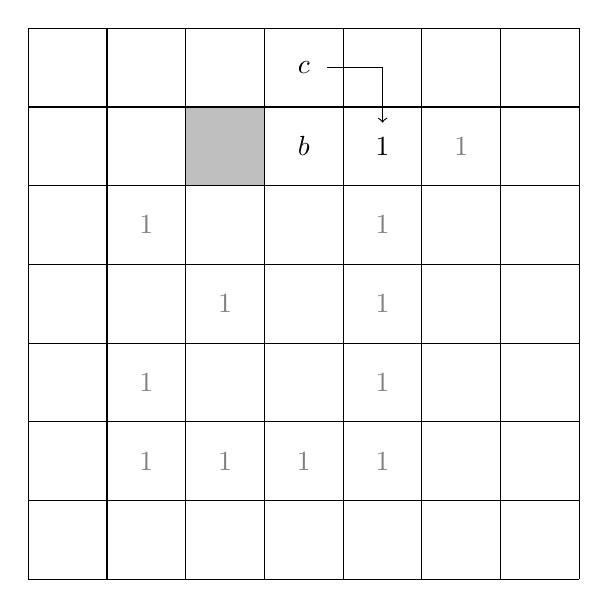
\begin{tikzpicture}

\foreach \x in {0,...,7} {
	\draw (\x,0) -- (\x,7);
	\draw (0,\x) -- (7,\x);
}

\draw[fill=lightgray] (2,5) rectangle (3,6);
\node at (3.5,6.5) {$c$};
\node at (3.5,5.5) {$b$};
\node at (4.5,5.5) {1};
\foreach \x/\y in {1/1,1/2,2/3,1/4,5/5,4/4,4/3,4/2,4/1,3/1,2/1} {
	\node [gray] at  (\x+0.5,\y+0.5) {1};
}
\draw [->] (3.8,6.5) -- (4.5,6.5) -- (4.5,5.8);

\end{tikzpicture}